\documentclass{homework}
\title{Homework 3}
\begin{document}
\maketitle

\begin{problem}
We recall the definition of divided differences for convenience:
\[f[x_0] = f(x_0), \quad f[x_0,\vec x,x_n] = \frac{f[\vec x,x_n] - f[x_0,\vec x]}{x_n - x_0}.\]
\begin{enumerate}[label=(\roman*)]
\item We argue by induction. For \(m=0\) this is obvious. Suppose this holds for \(m-1\), then we expand the definition:
\[\begin{aligned}
f[x_0,\vec x,x_m]
&= \frac{f[\vec x,x_m] - f[x_0,\vec x]}{x_m - x_0}\\
&= \frac{1}{x_m-x_0} \left[\sum_{i=1}^{m} \frac{f(x_i)}{\prod_{1\le j \le m}^{j\ne i}(x_i-x_j)} - \sum_{i=0}^{m-1} \frac{f(x_i)}{\prod_{0\le j \le m-1}^{j\ne i}(x_i-x_j)}\right]\\
&= \frac{1}{x_m-x_0} \left[\sum_{i=0}^{m} \frac{f(x_i)(x_i-x_0)}{\prod_{0\le j \le m}^{j\ne i}(x_i-x_j)} - \sum_{i=0}^{m} \frac{f(x_i) (x_i-x_m)}{\prod_{0\le j \le m}^{j\ne i}(x_i-x_j)}\right]\\
&= \frac{1}{x_m-x_0} \sum_{i=0}^m \frac{f(x_i) (x_m - x_0)}{\prod_{0\le j\le m}^{j\ne i} (x_i-x_j)}\\
&= \sum_{i=0}^m \frac{f(x_i)}{\prod_{0\le j\le m}^{j\ne i} (x_i-x_j)}.
\end{aligned}\]
\item Problem 1.(i) already gives a permutation-invariant way to express divided differences. The denominator is always the coordinate of this node minus all the other nodes, multiplied together.
\item We apply the definition, and by (ii) we reorder the nodes to put \(x_k\) at the beginning.\qed
\end{enumerate}
\renewcommand{\qed}{}
\end{problem}

\begin{problem} The Chebyshev nodes are
\(x_k = \cos \frac{(2k+1)\pi}{2n+2}\) for \(0 \le k \le n\).
\begin{enumerate}[label=(\roman*)]
\item There are \(N(a,b) = \lfloor \frac{(b+1)(n+1)}{2} \rfloor - \lceil \frac{(a+1)(n+1)}{2} \rceil\) points in the interval, by elementary considerations. Since \(\lfloor x \rfloor = x + O(1)\), we conclude that
\[\begin{aligned}
\lim_{n\to\infty} \frac{N(a,b)}{n+1}
&= \lim_{n\to\infty} \frac1{n+1} \left[\frac{(b+1)(n+1)}{2} - \frac{(a+1)(n+1)}{2} + O(1)\right]\\
&= \lim_{n\to\infty} \frac{b-a}{2} + O(1/n) = \frac{b-a}{2}.
\end{aligned}\]
\item We need to count the points with \[a \le \cos \frac{(2k+1)\pi}{2n+2} \le b.\] So we apply \(\arccos\) which is monotonic decreasing:
\[\arccos b \le \frac{2k+1}{2n+2} \pi \le \arccos a.\] So there are
\[N(a,b) = \left\lfloor \frac{n+1}{\pi}\arccos a -\frac 12\right\rfloor - \left\lceil \frac{n+1}{\pi}\arccos b -\frac 12\right\rceil.\]
By the same estimation we have
\[\lim_{n\to\infty}\frac{N(a,b)}{n+1} = \frac{\arccos a - \arccos b}{\pi}.\]
\item We take \(a = x\), \(b = x + \epsilon\). Since the fraction of points in the interval \([a,b]\) approaches \(\eta(a,b) = \frac{\arccos a - \arccos b}{\pi}\), we calculate the density
\[\lim_{\epsilon\to0}\frac{\eta(x,x+\epsilon)}{\epsilon} = -\frac1\pi \arccos' x = \frac{1}{\pi \sqrt{1-x^2}},\] as desired. \qed
\end{enumerate}
\renewcommand{\qed}{}
\end{problem}

\begin{problem} We have \(T_k(x) = \cos (k\arccos x)\).
\begin{enumerate}[label=(\roman*)]
\item The derivative of a Chebyshev polynomial is
\[T'_k(x) = \frac{k\sin(k\arccos x)}{\sqrt{1-x^2}}.\] Substituting the Chebyshev nodes, we have
\[T'_{n+1}(x_j) = \frac{(n+1)\sin \frac{ (2j+1)\pi}{2}}{\sin\frac{(2j+1)\pi}{2n+2}} = (-1)^{j}(n+1)\csc\frac{(2j+1)\pi}{2n+2}.\]
Therefore by trigonometric identities
\[T'_{n+1}(x_j) - T'_{n-1}(x_j) = \begin{cases}
2n(-1)^j & 1 \le j \le n-1\\
4n(-1)^j & j = 0 \lor j = n.
\end{cases}\]
\item By the Leibniz derivative rule we have
\[l'(x) = \sum_{i=0}^n \prod_{k\ne i} (x - x_k).\]
Substituting \(x = x_j\), we see that all terms except one contain \((x_j - x_j)\) and vanish. We are left with \(\prod_{k\ne j} (x_j - x_k)\). This shows \(\lambda_j = 1/l'(x_j)\).
\item For Chebyshev nodes, \(l(x) = 2^{1-n}T_n(x)\). Therefore using (ii) we only need to evaluate \(T'_n(x_j)\). We have the recurrence relation
\[T_{n+1}(x) = 2xT_n(x) - T_{n-1}(x),\]
Differentiating we have
\[T'_{n+1}(x) = 2T_n(x) + 2xT'_n(x) - T'_{n-1}(x).\]
Substituting \(x = x_j\) we see that \(T_n(x_j)\) vanishes. Recalling the results from (i) and after some elementary computation we are left with
\[T_n'(x_j) = (-1)^{j}n\]
and twice the result for \(j = 0, n\). Combining these we showed the desired equation.
\item \emph{On calcule!}
\[\begin{aligned}
\prod_{k\ne j} (x_j - x_k)
&= \prod_{k\ne j} \frac{2(j-k)}{n+1}\\
&= h^{n-1}\prod_{k \le j} (j-k) \cdot \prod_{k\ge j} (j-k)\\
&= (-1)^{n-j} h^{n-1} j! (n-j)!
\end{aligned}\]
which after taking the reciprocal, agrees with the result. \qed
\end{enumerate}
\renewcommand{\qed}{}
\end{problem}

\begin{problem}
We first set up some global variables, and compute the Chebyshev nodes:
\begin{matlab}
global Xs n xs;
Xs = (-1 : 0.01 : 1);

n = 20;
xs = cos((0:n-1) * pi / (n-1));
\end{matlab}
We implement the barycentric interpolation using the explicit formula for weights. Note that we didn't account for the case where \(x = x_i\) coincides with one of the nodes. In this case the algorithm should return \texttt{Inf / Inf = NaN}, which will not show up on the graph.
\begin{matlab}
function y = barycentric(ys, x)
  global n xs;
  dx = (-1) .^ (0:n-1) ./ (x - xs);
  dx([1;n]) = dx([1;n]) ./ 2;
  y = sum(ys .* dx) / sum(dx);
end
\end{matlab}
And finally a helper function that plots the difference for us:
\begin{matlab}
function interpolate(f)
  global xs Xs;
  ys = arrayfun(f, xs);
  plot(Xs, arrayfun(@(x) barycentric(ys, x) - f(x), Xs));
end
\end{matlab}
For instance, the difference for the function \(f(x) = |x|\) using 20 nodes is shown below.
\begin{center}
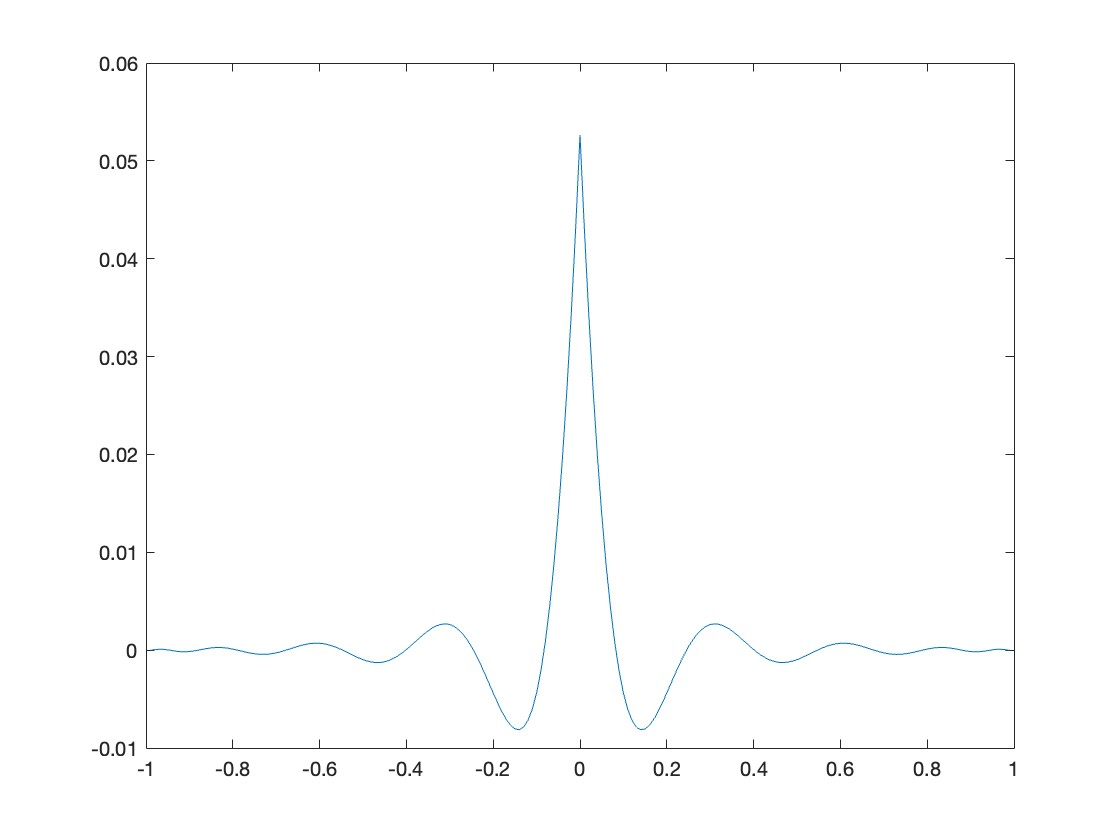
\includegraphics[width=0.7\textwidth]{Hw3-Fig1.jpg}
\end{center}

For the function \(f(x) = \tanh(50\pi x)\), the closest singularity is at \(x = \pm \frac{i}{100}\). Since the semi-minor axis of the Bernstein ellipse \(E_\rho\) is \(\frac{\rho - \rho^{-1}}{2}\), we solve that \(\rho = \frac{\sqrt{10001} + 1}{100} \approx 1.01005\).
This means the Chebyshev interpolations satisfy
\[|f - p_n| \le \frac{4 M \rho^{-n}}{\rho - 1}
\approx 400 \times 1.01^{-n}.\]
We verify our predictions below.

We choose \(f_1(x) = |x|\), \(f_2(x) = x|x|\), and \(f_3(x) = e^{-3x^2}\). This results in the following error graph:
\begin{center}
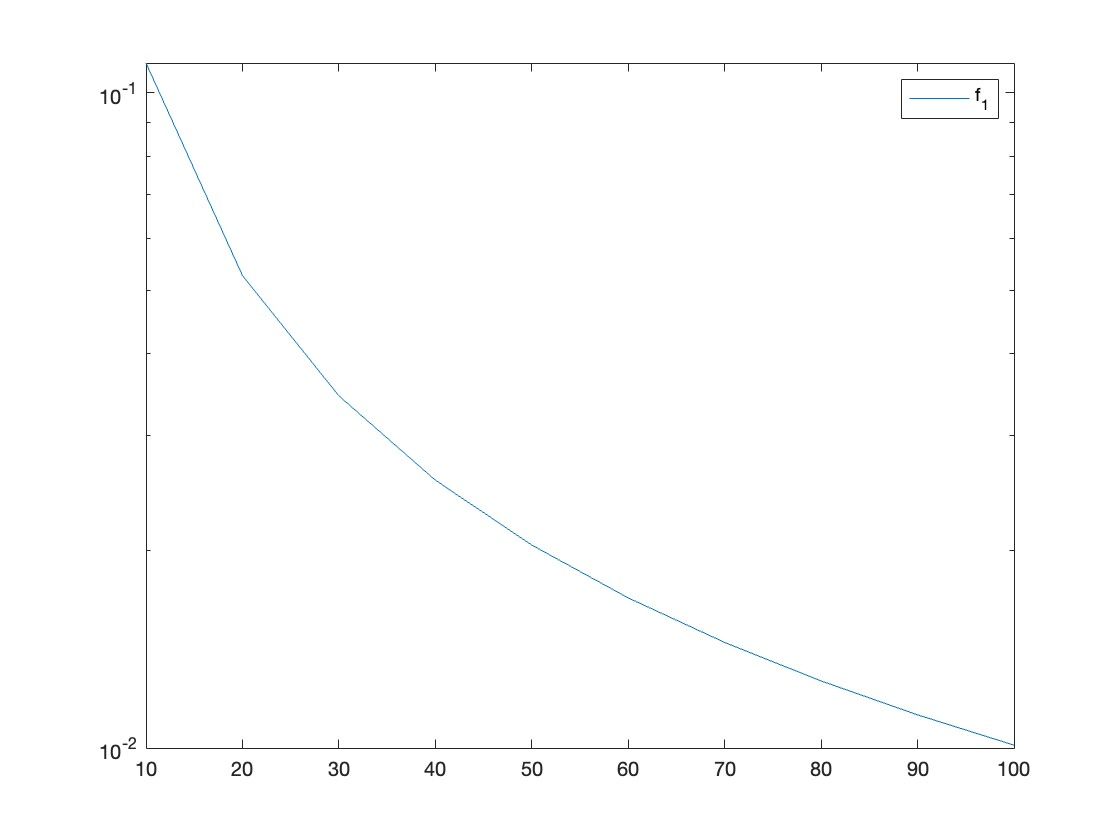
\includegraphics[width=0.45\textwidth]{Hw3-Fig2-1.jpg}
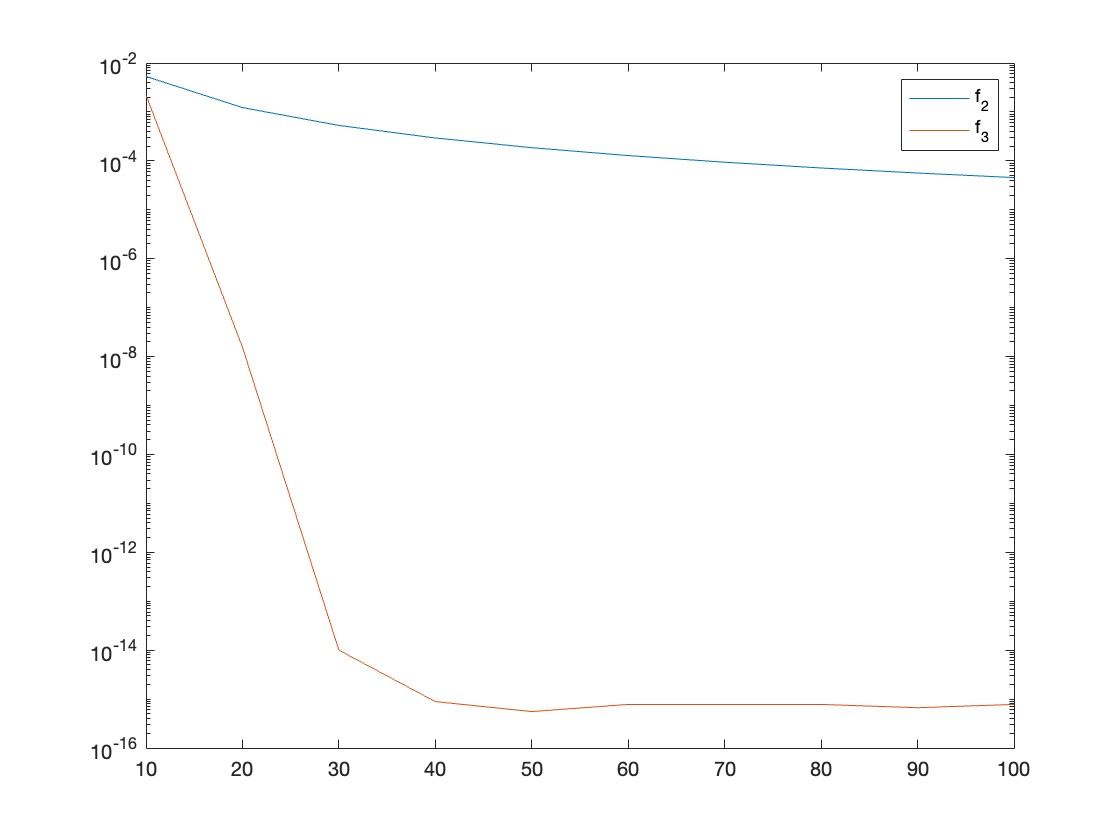
\includegraphics[width=0.45\textwidth]{Hw3-Fig2-2.jpg}
\end{center}
It is seen that differentiable functions generally converge faster. Finally we look at \(\tanh(50\pi x)\).
\begin{center}
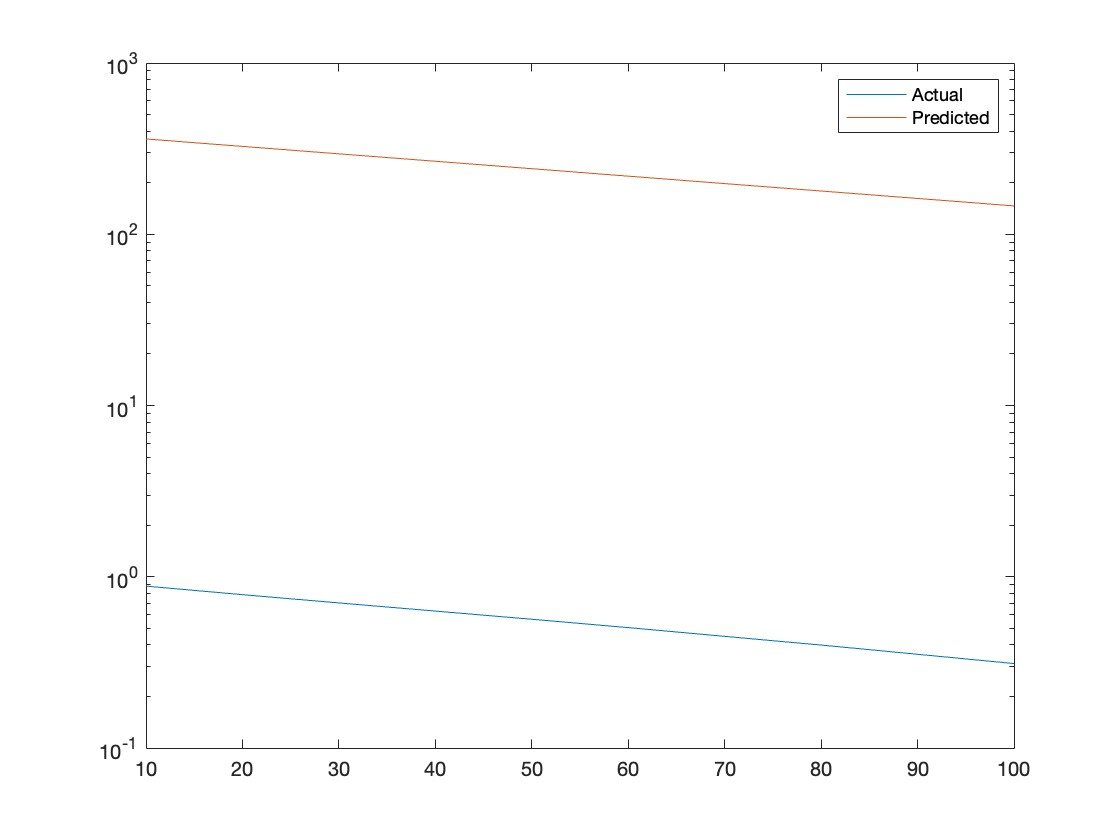
\includegraphics[width=0.7\textwidth]{Hw3-Fig3.jpg}
\end{center}
The lines are almost parallel, so our predictions are correct up to a constant. And since this is an upper bound, the prediction is indeed higher than the actual error. However it is off by a few hundred times, which probably means that \(\tanh\) is relatively well-behaved.
\end{problem}

\begin{problem}
We have \(h = \frac2{n+1}\), plugging into the previous results we get
\[\frac{\lambda_{n/2}}{\lambda_n} = \frac{(-1)^{n/2}h^{n-1} (\frac n2)! (\frac n2)!}{(-1)^0 h^{n-1} n!} = (-1)^{n/2} {n \choose \frac n2}.\]
This ratio grows as \(O(4^n / \sqrt n)\), which is very fast. Therefore for a generic \(x\), the factor \(\lambda_{n/2}/\lambda_n\) will dominate the factor \((x - x_{n/2})/(x-x_n)\), thus by the second form of the barycentric formula, the polynomial will be much more sensitive to changes of the center datapoint compared to the endpoints.
\end{problem}

\newpage
\section*{Appendix: Souce Code}
Code can also be found at 
\begin{center}
\texttt{https://github.com/Trebor-Huang/Numerical-Analysis-Homework}
\end{center}
\matlabfile{Hw3.m}

\end{document}
